\documentclass[10pt]{article}

\usepackage{caption}
\usepackage{subcaption}
\usepackage{subfig}
\usepackage{graphicx}
\usepackage{multirow}
\usepackage{wrapfig}
\usepackage{enumerate}
\usepackage{amsmath}
\usepackage{tabularx}
\usepackage[margin=1.1in]{geometry}

\providecommand{\e}[1]{\ensuremath{\times 10^{#1}}}

\begin{document}

\section{Exercise 1: SVM}

In the general case of solving a linear SVM with slack variables without a regularizer, the objective function is:

\begin{subequations}
\begin{align}
	\underset{\alpha}{\text{minimize}}
		& \quad -\sum_{i = 1}^n \alpha_i + \frac{1}{2} \sum_{i = 1}^n \sum_{j = 1}^n \alpha_i \alpha_j y^{(i)} y^{(j)} (x^{(i)} \cdot x^{(j)}) \\
	\text{subject to}
		& \quad 0 \leq \alpha_i \leq C \quad \forall i \,, \\
		& \quad \sum_{i = 1}^n \alpha_i y^{(i)} = 0
\end{align}
\label{eq:singlesvm}
\end{subequations}

Using the Python CVXOPT package, the general form of the objective function is:

\begin{subequations}
\begin{align}
	\underset{x}{\text{minimize}}
		& \quad \frac{1}{2}x^T P x + q^T x \\
	\text{subject to} 
		& \quad Gx \leq h \\
		& Ax = b
\end{align}
\label{eq:cvxopt}
\end{subequations}

The general form for converting our slack variable objective function in Equation \ref{eq:singlesvm} to the CVXOPT objective function in Equation \ref{eq:cvxopt} is described in Table \ref{tbl:cvxopttosvm}.

\begin{table}[!ht]
\centering
\begin{tabular}{c|p{.7\textwidth}}
	CVXOPT& Conversion from Equation \ref{eq:singlesvm} \\ \hline
	$x$ & If there are $n$ points in the training set, an $n \times 1$ vector equal to the values of $x$ in the training data \\
	$P$ & An $n \times n$ matrix which is the kernel matrix between all pairs of training data $x$ weighted by the corresponding value of $y$ from the training data \\
	$q$ & An $n \times 1$ vector of $-1$s \\
	$G$ & A $2n \times n$ matrix where the top $n \times n$ is the identity matrix and the bottom $n \times n$ is the negative identity matrix \\
	$h$ & A $2n \times 1$ vector with the top $n \times 1$ vector of $C$s and the bottom $n \times 1$ vector of $0$s \\
	$A$ & An $1 \times n$ vectors with elements $y^{(i)}$ from the training set for all values of $i$ \\
	$b$ & An $1 \times 1$ vector of $0$s
\end{tabular}
\caption{Conversion rule for deriving CVXOPT constraints}
\label{tbl:cvxopttosvm}
\end{table}

For the small example with $(1,2),(2,2)$ as positive examples and $(0,0),(-2,3)$ as negative examples, the constraints from CVXOPT as written above are written in Equation \ref{eq:1-1}.

\begin{subequations}
\begin{align*}
	P &= \begin{bmatrix}
		5 & 6 & 0 & -4 \\
		6 & 8 & 0 & -2 \\
		0 & 0 & 0 & 0 \\
		-4 & -2 & 0 & 13
	\end{bmatrix} 
	&& q = \begin{bmatrix}
		-1 \\ -1 \\ -1 \\ -1
	\end{bmatrix} \\
	G &= \begin{bmatrix}
		1 & 0 & 0 & 0 \\
		0 & 1 & 0 & 0 \\
		0 & 0 & 1 & 0 \\
		0 & 0 & 0 & 1 \\
		-1 & 0 & 0 & 0 \\
		0 & -1 & 0 & 0 \\
		0 & 0 & -1 & 0 \\
		0 & 0 & 0 & -1
	\end{bmatrix} 
	&& h = \begin{bmatrix}
		1 \\ 1 \\ 1\\ 1\\ 0\\ 0\\ 0\\ 0
	\end{bmatrix}\\
	A &= \begin{bmatrix}
		1 & 1 & -1 & -1	
	\end{bmatrix} 
	&& b = \begin{bmatrix}
		0
	\end{bmatrix}
\end{align*}
\label{eq:1-1}
\end{subequations}

The decision boundary generated by the SVM code for the small example is shown in Figure \ref{fig:1-1}.

\begin{figure}[!ht]
\centering
\begin{subfigure}[b]{0.46\textwidth}
	\centering
	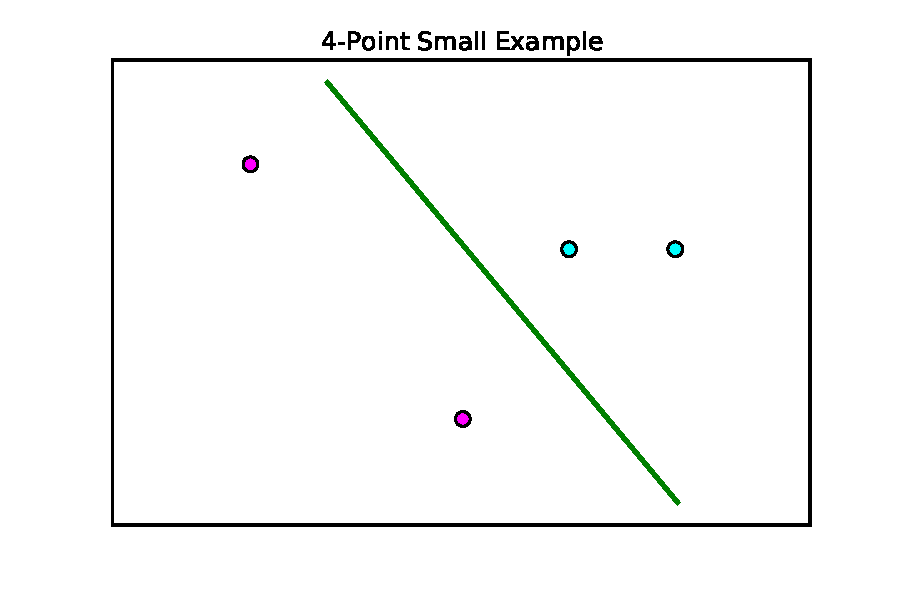
\includegraphics[width=\textwidth]{exercise1-1.pdf}
	\caption{Decision boundary for 4 points using CVXOPT and SVM with slack variables}
	\label{fig:1-1}
\end{subfigure}
\begin{subfigure}[b]{0.46\textwidth}
\centering
\begin{tabular}{r|c|c|c}
	Dataset & Kernel & Training & Validation \\ \hline
	smallOverlap & Linear & $.24$ & $.24$ \\
	smallOverlap & Gaussian $\beta = 0.1$ & $.26$ & $.25$ \\
	smalloverlap & Gaussian $\beta = 1$ & $.26$ & $.25$ \\
	bigoverlap & linear & $.305$ & $.255$ \\
	bigoverlap & Gaussian $\beta = 0.1$ & $.3$ & $.255$ \\
	bigoverlap & Gaussian $\beta = 1$ & $.3$ & $.255$ \\
	ls & linear & $0$ & $0.00375$ \\
	ls & Gaussian $\beta = 0.1$ & $0.0625$ & $0.0775$ \\
	ls & Gaussian $\beta = 1$ & $0.0625$ & $0.0775$ \\
	nonsep2 & linear & $.485$ & $.495$ \\
	nonsep2 & Gaussian $\beta = 0.1$ & $.48$ & $.4975$ \\
	nonsep2 & Gaussian $\beta = 1$ & $.48$ & $.4975$ \\
	stdev1 & Gaussian $\beta = 0.5$ & $0$ & $.005$ \\
	stdev1 & Gaussian $\beta = 1$ & $0$ & $.005$
\end{tabular}
\caption{Error rates for training and validation sets, $c = 1$, linear and Gaussian kernels}
\label{tbl:1-2-error}
\end{subfigure}
\end{figure}

\begin{figure}[!ht]
\centering
\begin{subfigure}[b]{0.46\textwidth}
	\centering
	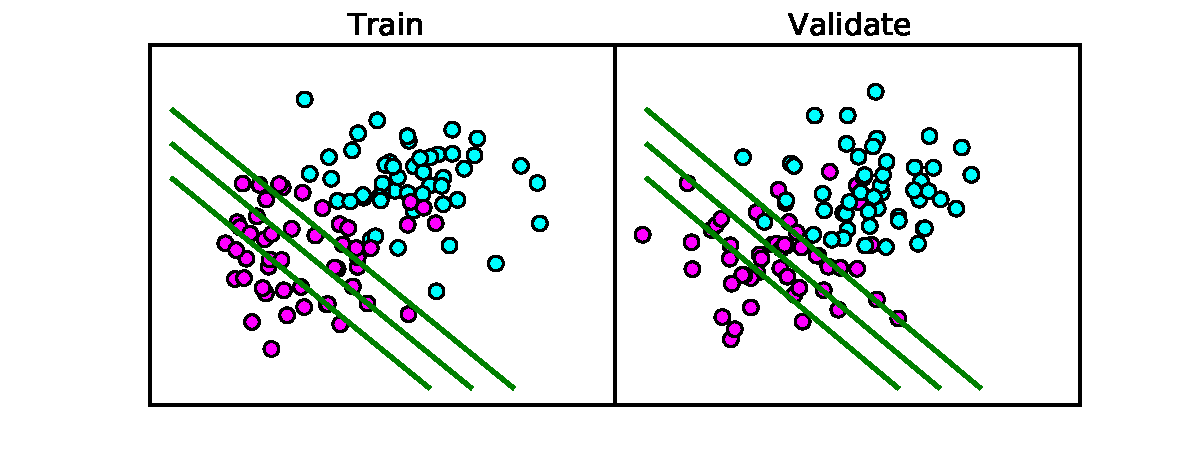
\includegraphics[width=\textwidth]{1-2-smallOverlap.pdf}
	\caption{smallOverlap}
	\label{fig:1-2-smalloverlap}
\end{subfigure}
\begin{subfigure}[b]{0.46\textwidth}
	\centering
	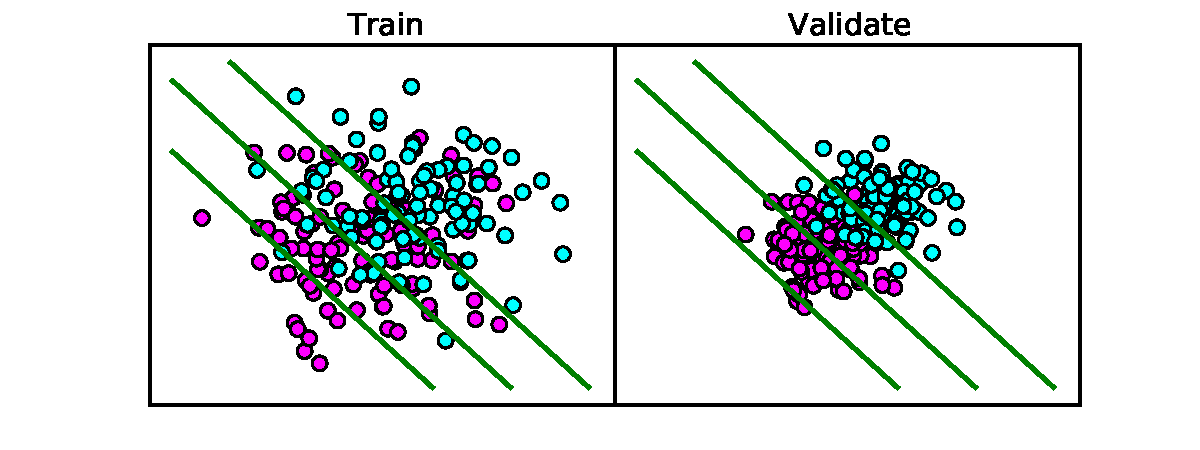
\includegraphics[width=\textwidth]{1-2-bigOverlap.pdf}
	\caption{bigOverlap}
	\label{fig:1-2-bigoverlap}
\end{subfigure}
\\
\begin{subfigure}[b]{0.46\textwidth}
	\centering
	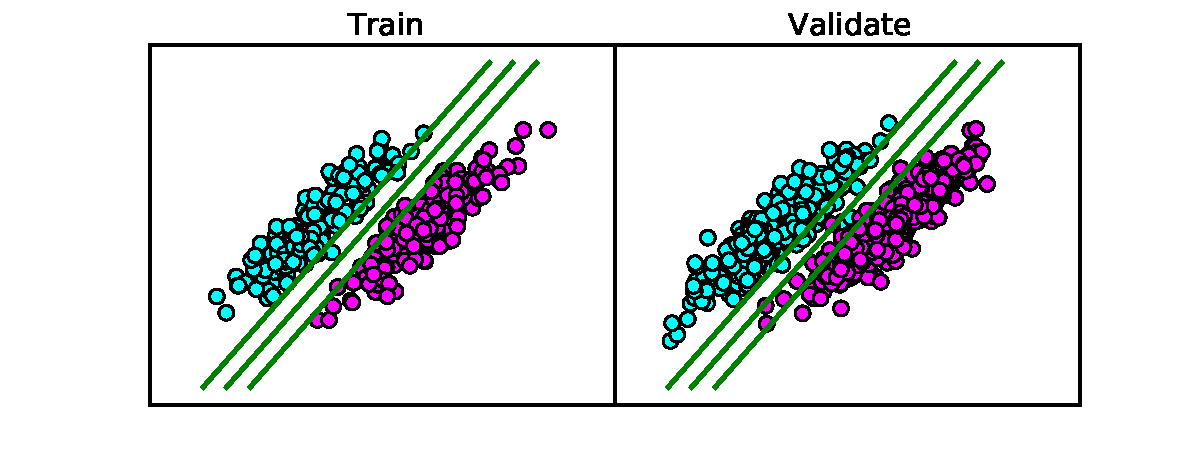
\includegraphics[width=\textwidth]{1-2-ls.pdf}
	\caption{ls}
	\label{fig:1-2-ls}
\end{subfigure}
\begin{subfigure}[b]{0.46\textwidth}
	\centering
	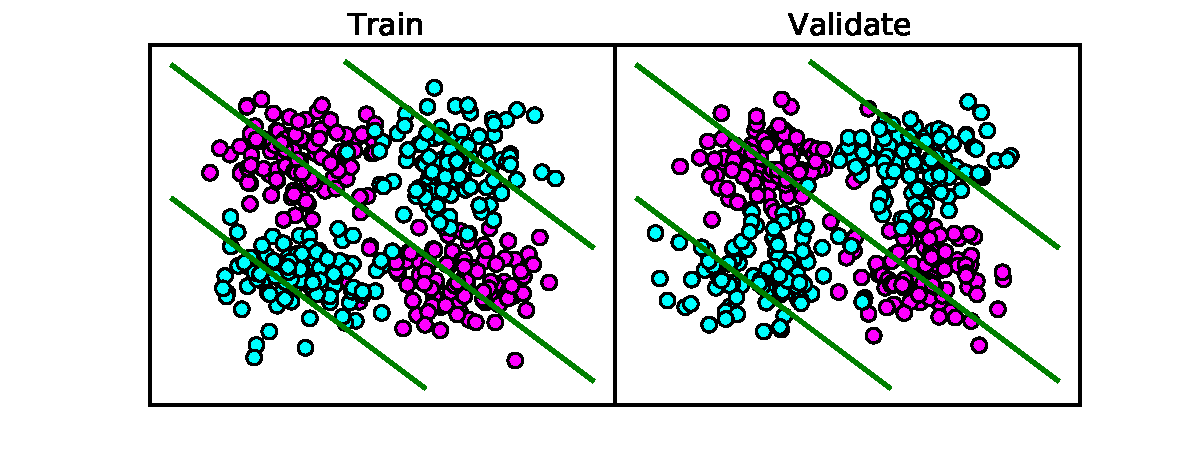
\includegraphics[width=\textwidth]{1-2-nonSep2.pdf}
	\caption{nonSep2}
	\label{fig:1-2-nonSep2}
\end{subfigure}
\end{figure}

Setting $C = 1$, the error rates for the training and validation sets for different data sets and kernels is shown in Table \ref{tbl:1-2-error}. If a data set did not come with a training / validation set pair, the dataset was randomly cut in half for each class to use as training and validation. In general, the more separable the data set is, the better the slack-variable SVM without a regularizer does. In the non-separable case, depending on the nature of the inseparability, the solution has a higher error rate.

Using a Gaussian kernel at different bandwidths does not change the error rates much unless the data is distributed with a Gaussian distribution, as shown in Table \ref{tbl:1-2-error}.

\begin{figure}[!ht]
\centering
\begin{subfigure}[b]{0.46\textwidth}
	\centering
	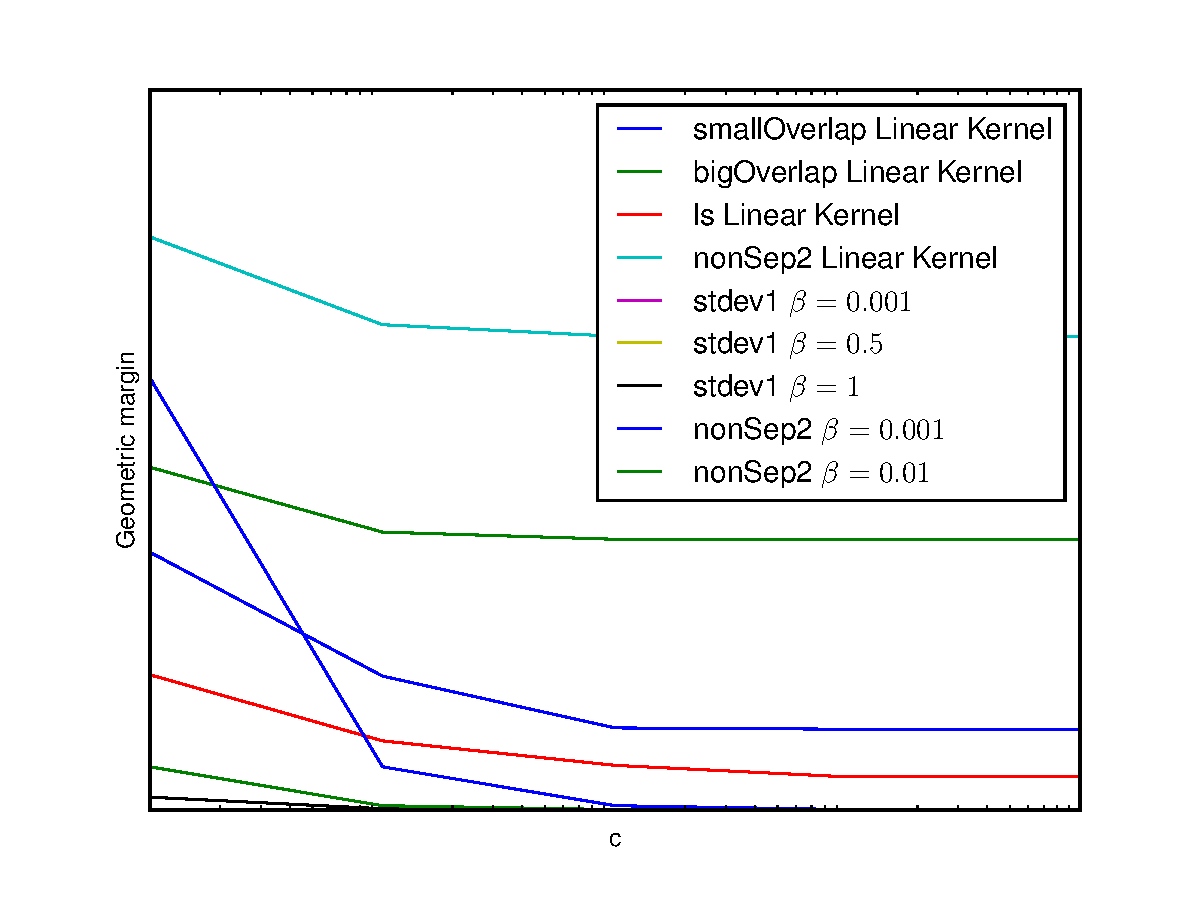
\includegraphics[width=\textwidth]{1-3-c-margin.pdf}
	\caption{plot of the geometric margin as a function of $c$ for various kernels and datasets}
	\label{fig:1-3-c-margin}
\end{subfigure}
\begin{subfigure}[b]{0.46\textwidth}
	\centering
	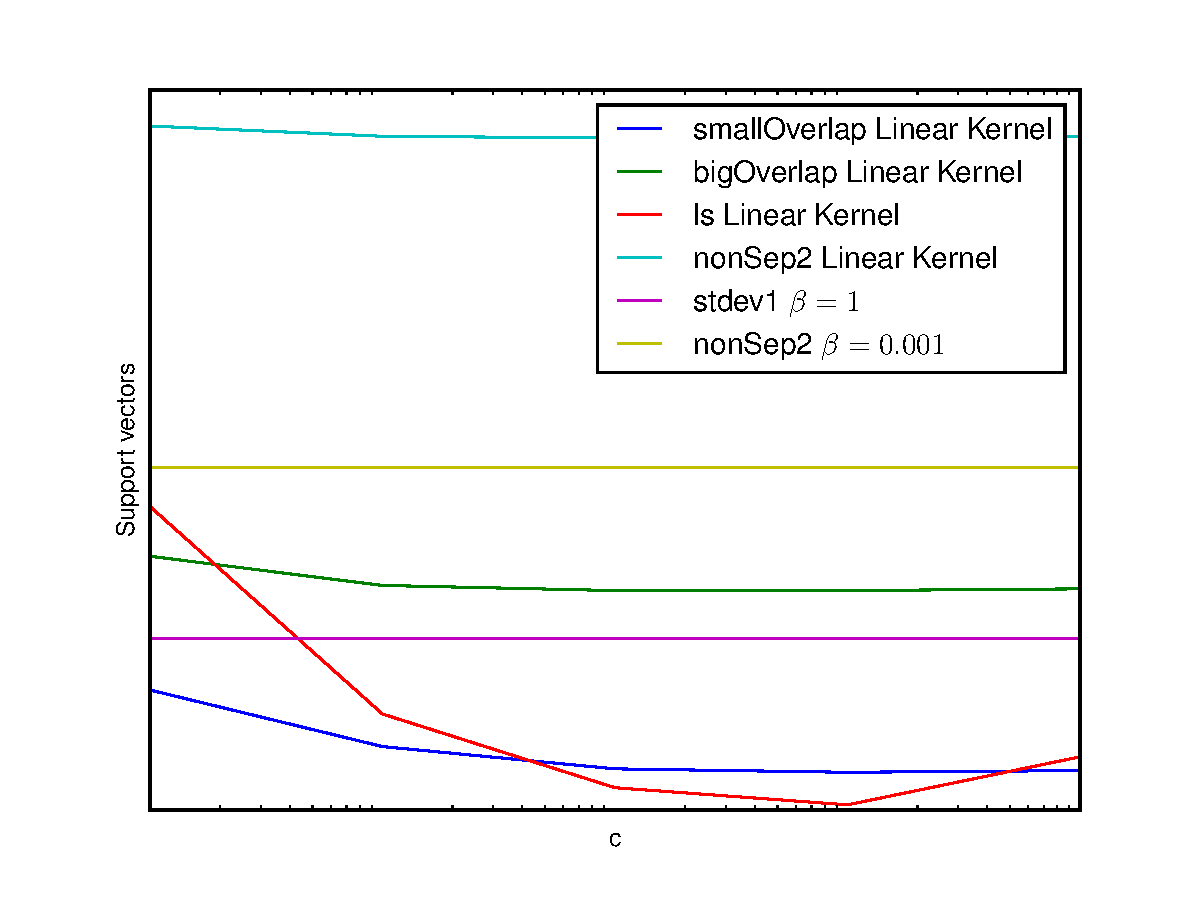
\includegraphics[width=\textwidth]{1-3-support-vectors.pdf}
	\caption{plot of the number of support vectors as a function of $c$ for various kernels and datasets}
	\label{fig:1-3-support-vectors}
\end{subfigure}
\end{figure}

As $c$ increases, the geometric margin decreases, as shown for various values of $c$, various kernels, and various datasets in figure \ref{fig:1-3-c-margin}. this always happens as $c$ increases, because this means there can be more slack in the final svm, which means the svm will be more tolerable to incorrect classifications for inseparable data. the number of support vectors first decreases, then increases as $c$ increases, as shown in figure \ref{fig:1-3-support-vectors}. this means that the classifier is less overfit on the training data and will have smaller errors on the testing data. choosing $c$ for maximizing the margin will yield a value of $c$ equal to zero, which is the same as having a hard-margin svm that does not perform well on non-separable data. an alternate criteria for choosing $c$ could be the minimum number of support vectors (since the number of support vectors eventually increases with a higher value of $c$ as the classifier gets over-fit to the training data). Changing $c$ has almost no effect on the training error unless the data is highly non-separable.

\section{Exercise 2: logistic regression}

The kernelized form of the regression objective for logistic regression having all data with $y^{(i)} \in {-1, 1}$ is written in Equation \ref{eq:kernelized-lr}. $K$ is the kernel function, which in the linear case is $x^{(i')} \cdot x^{(i)}$. For accurate results, it was important to set the tolerance of the solver to $1\e^{-12}$

\begin{subequations}
	\begin{align}
		\text{NLL}(\alpha, w_0) = \sum_i \log \left(1 + e^{-y^{(i)}\left(\displaystyle\sum_{i'} \alpha_{i'} K(x^{(i')}, x^{(i)}) + w_0\right)}\right)
	\end{align}
	\label{eq:kernelized-lr}
\end{subequations}

% \begin{figure}[!ht]
% \begin{subfigure}[b]{0.46\textwidth}
% 	\centering
% 	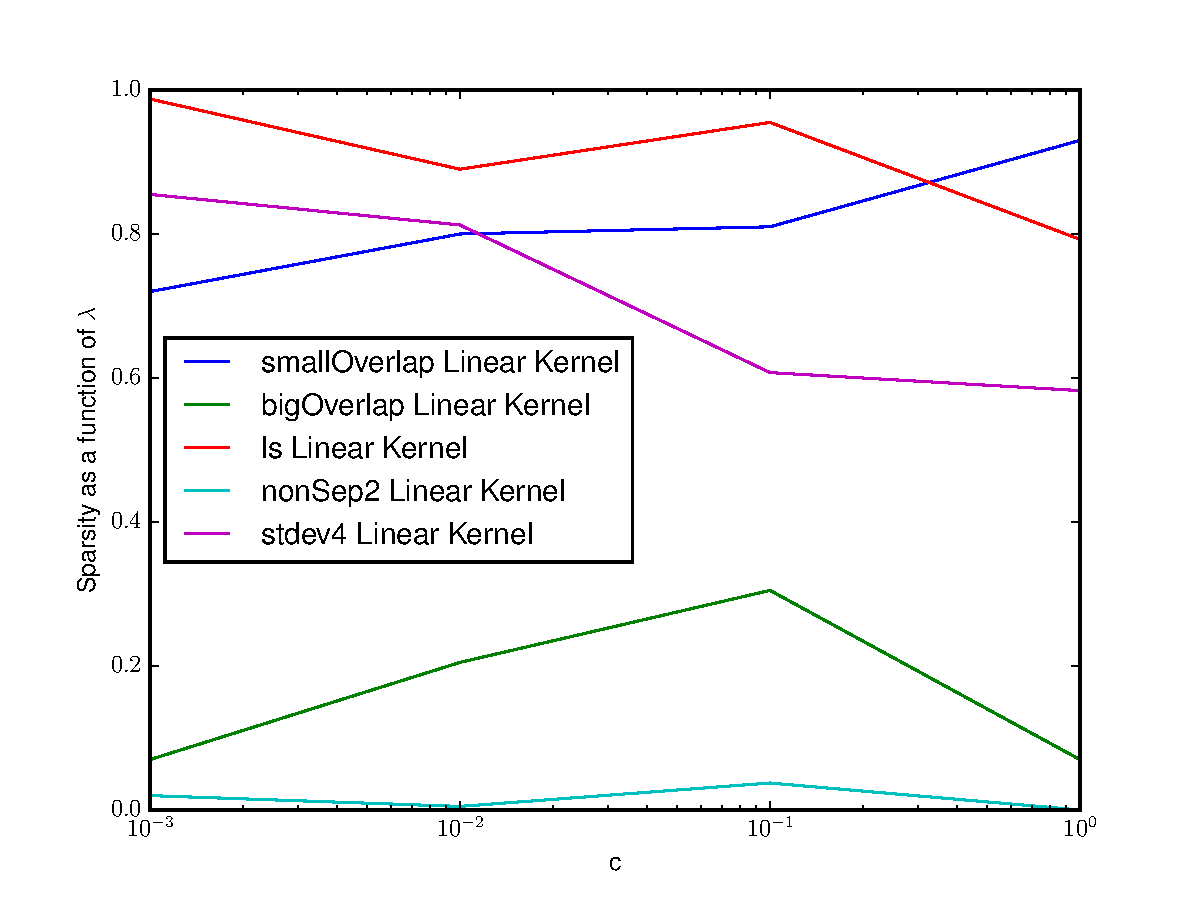
\includegraphics[width=\textwidth]{exercise2-2.pdf}
% 	\caption{ls}
% 	\label{fig:2-2}
% \end{subfigure}
% \begin{subfigure}[b]{0.46\textwidth}
% 	\centering
% 	\includegraphics[width=\textwidth]{exercise2-3.pdf}
% 	\caption{nonSep2}
% 	\label{fig:2-3}
% \end{subfigure}
% \end{figure}

Here I am defining sparsity as the percentage of points in the training data that are used as support vectors (with alpha values greater than $1\e^{-5}$. Using L1 regularization with parameter $\lambda$ on the $\alpha$ values to ensure sparsity, the relationship between $\lambda$ and sparsity is shown in Figure \ref{fig:2-2}. In general, the sparsity follows a U-pattern, sometimes in two places, as $\lambda$ increases. The optimal value of $\lambda$ is the one that in the separable case makes the sparsity the lowest for the smallest value of $\lambda$. As $\lambda$ gets too large, the error on the training and testing sets increases too much, so it is better to choose a smaller value of $\lambda$ that allows for low training / testing error. 


Gaussian kernels in general work much better on non-separable data. SHOW A GRAPH HERE.

2.2: 
* do training set over some values of lambda
* use that to pick lambda based on sparsity
* test on `validation' data and report an error value

2.3:
will need to plot lambda versus sparsity

2.4:
* do training set over some values of bandwidth with lambda = 0
* do validation set over some values of lambda
* test on test and report results

2.5:
* will need to think about this a little bit more.

3.1:
* https://piazza.com/class/hzdfawvtilo7hf?cid=434
* l2 regularization, linear case
* http://blog.datumbox.com/machine-learning-tutorial-the-multinomial-logistic-regression-softmax-regression/

* maybe need to save coefficients or predictions or something?

3.1 - lr:
* 2 features, 100 pts, 2 classes, l = 0.01 -> error = .485
* might need to randomly select subsets of data points

* bigoverlap - error is .26 on test, ,.305 on training with l = 0.1
* smalloverlap - error is .26 on test, .27 on training with l = 0.1

* tips for getting numerics to work better:
	* normalize data beforehand (then don't forget to re-normalize later)
	* 

3.2 - multiclass svm:
* used http://scikit-learn.org/stable/modules/generated/sklearn.svm.linearsvc.html
* can do this so fast it doesn't even make sense to try to do this by myself.
* tried an array of l values with l1 loss (multiclasssvm.py), best l with random partitioning of data into 3 sets. rigorous stopping criteria
* hinge loss, l2 regularization: 
	* validation error: .187
	* test error: .261
	* l: 0.01
* squared loss, l1 regularization:
	* validation error: .143
	* test error: .143
	* l: 7e-7

\end{document}